\chapter{Commande longitudinale d'une maquette de DarkO}
\minitoc
\label{chap:3DOF}

\section{Motivation}
\label{sec:motivation3DOF}
Des simulations en boucle fermée avec le contrôleur \eqref{eq:u_hybrid} développé dans \ref{sec:ctrl_hyste} montrent qu'en présence d'un vent horizontal constant dans le plan $(x_{[b]},z_{[b]})$, le drone modifie son angle de tangage. Ce comportement a également été observé lors d'essais en soufflerie avec le dispositif expérimental \cite{olszaneckibarthHal-02542982}. Intuitivement, une réduction de l'angle d'attaque entraîne une diminution de la surface exposée au vent, de manière à réduire la force de traînée, ce qui a une forte incidence sur la position. Dans le même temps, le flux d'air dû au vent constant génère une portance, compensée par une réduction de la poussée de l'hélice et une réduction conséquente de la consommation du drone. L'objectif de la maquette décrite ici est d'évaluer expérimentalement l'effet du vent sur le dispositif DarkO.

De plus, il faut noter que le changement de l'angle d'attaque du drone a un impact sur la mesure du vent. Comme la sonde de Pitot est fixée sur le corps du drone, cette dernière se trouve être en rotation lors de la transition. On comprend donc que la mesure du vent ne sera valide qu'en vol d'avancement, à haute vitesse. En vol stationnaire ou lors de la transition, nous n'avons pas de mesure du vent, ni des rafales impactant le drone.

Nous allons donc proposer dans ce chapitre une méthode de commande n'utilisant pas de mesure de vent pour stabiliser le drone à une position de l'espace. Toutefois, nous commencerons par une stabilisation longitudinale sur une dynamique à trois degrés de liberté pour tester notre loi de commande.

\section{Présentation de la maquette expérimentale}
\label{sec:test_bench}



\subsection{Description physique, capteurs et actionnements}
Le prototype développé comprend des pièces imprimées en 3D, en Onyx et PLA  \nomenclature[]{\(PLA\)}{Thermoplastique : acide polylactique} (acide polylactique, un polyester thermoplastique). Le drone est spécialement conçu pour réaliser des expériences devant une soufflerie, avec un comportement semblable à celui de DarkO en raison de leur forme similaire (voir Fig. \ref{fig:real_test_bench}). La partie centrale, qui contient l'avionique embarqué (pilote automatique, GPS, etc.) dans DarkO, a été remplacée ici par un joint tournant à un degré de liberté (voir Fig. \ref{fig:rotation}). Les ailes sont les mêmes que celles du DarkO, avec les contrôleurs électroniques de vitesse (ESC), régissant la vitesse du moteur \textit{brushless}, placés dans les ailes.

Comme décrit dans la section \ref{sec:motivation3DOF}, nous souhaitons représenter et étudier le degré de liberté de l'axe $y_{\text{b}}$ du drone DarkO. Le tube principal en carbone reliant les deux ailes est utilisé comme axe de rotation. Ce tube est fixé sur deux roulements espacés de \SI{28.5}{\milli\meter} afin d'obtenir une fixation solide de l'ensemble. Cet axe de rotation est équipé d'un codeur optique rotatif en quadrature pour mesurer précisément l'orientation de l'appareil. L'avantage de ce capteur est qu'il ne produit pas de couple résistant sur l'axe de rotation. Ce codeur offre 4000 impulsions par tour, ce qui donne une résolution de $\SI{0.09}{\degree}/impulsion$.
\begin{figure}[!ht]
    \centering
    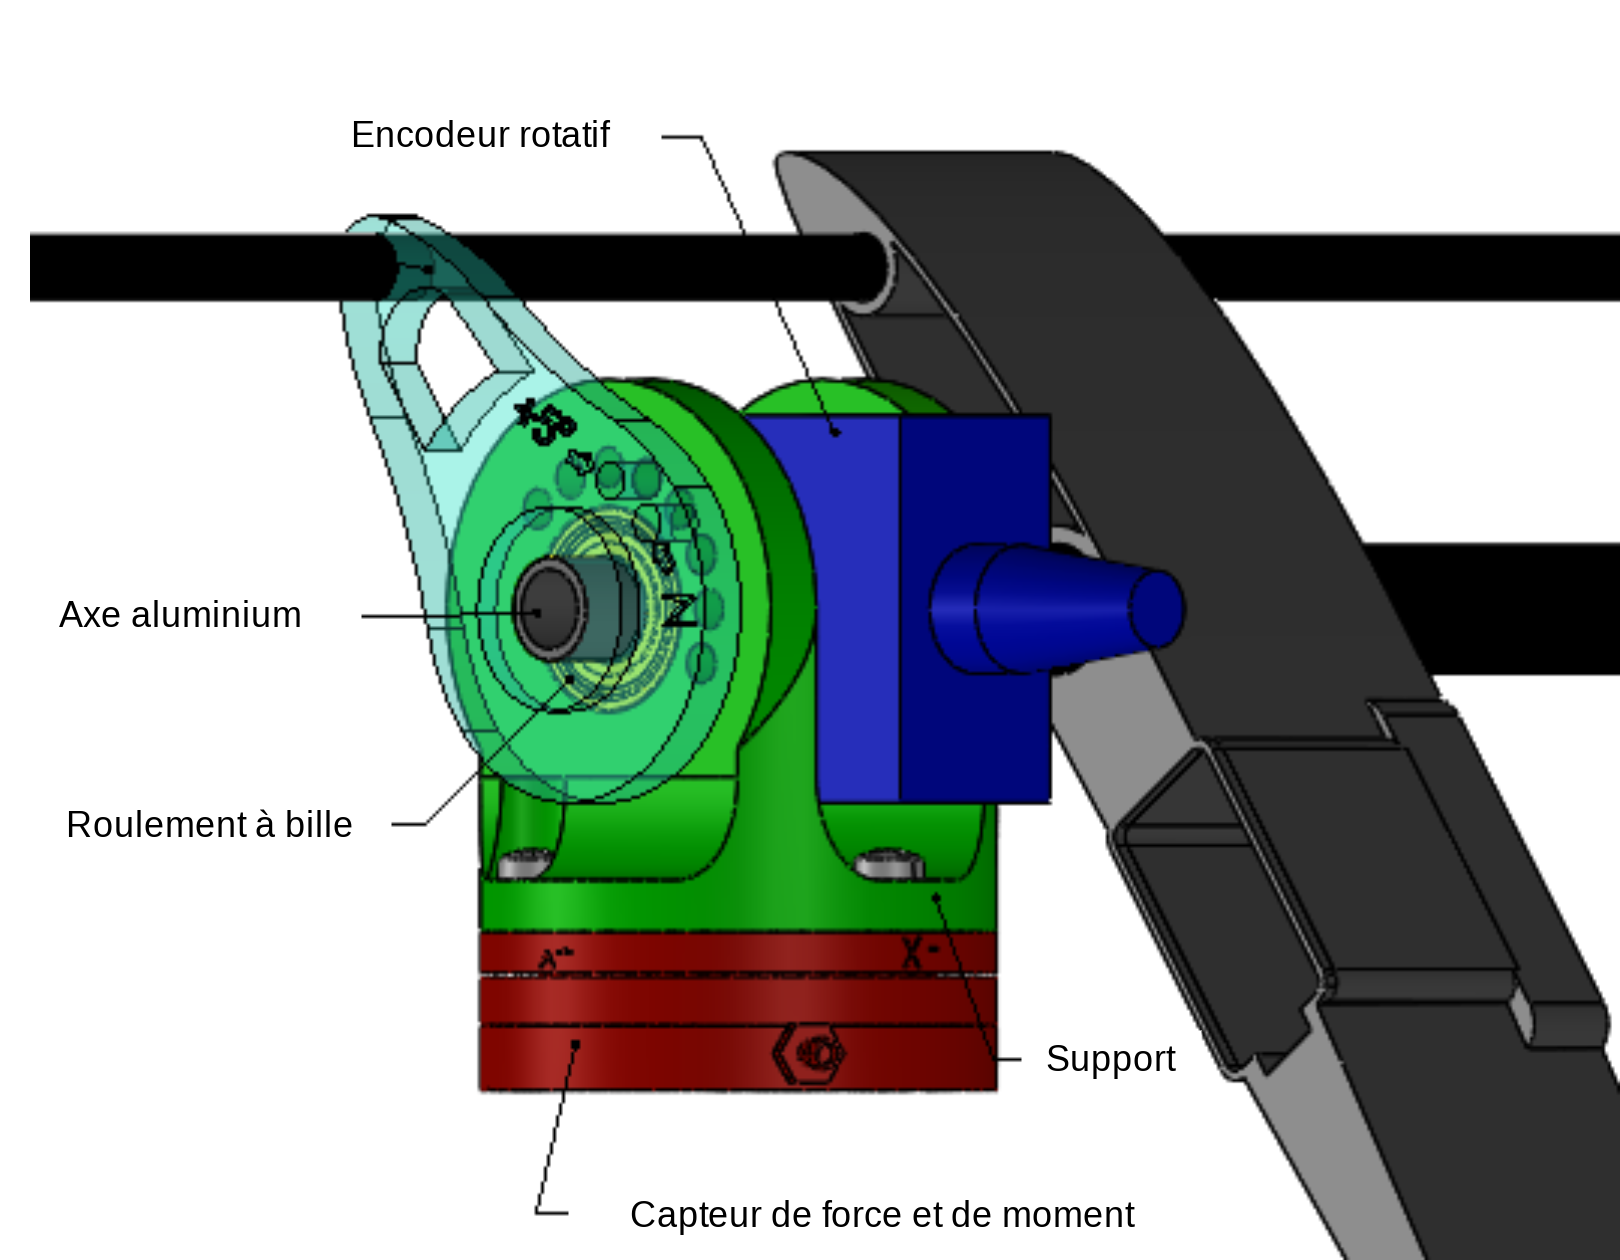
\includegraphics[width=0.6\columnwidth]{figures/MontageSupport2.png}.
    \caption{Montage à un degré de liberté.}
    \label{fig:rotation}
\end{figure} 

Comme le montre la figure \ref{fig:rotation}, l'indexeur et le support sont percés pour que la rotation puisse être bloquée, par une vis, à des positions connues ($0^\circ$, $90^\circ$, etc.). Le verrouillage de l'appareil permet une initialisation correcte de l'encodeur incrémental. Le verrouillage permet également de placer l'appareil dans des positions exactes spécifiques afin d'identifier les coefficients aérodynamiques. 

Le mécanisme est également équipé d'un capteur de forces et de moments à 6 degrés de liberté (DOF), qui permet de mesurer la force exercée sur le dispositif expérimental par le support. Le banc d'essai expérimental est également équipé d'un fil chaud pour mesurer la vitesse de l'air affectant la maquette. 

\begin{figure}[!ht]
    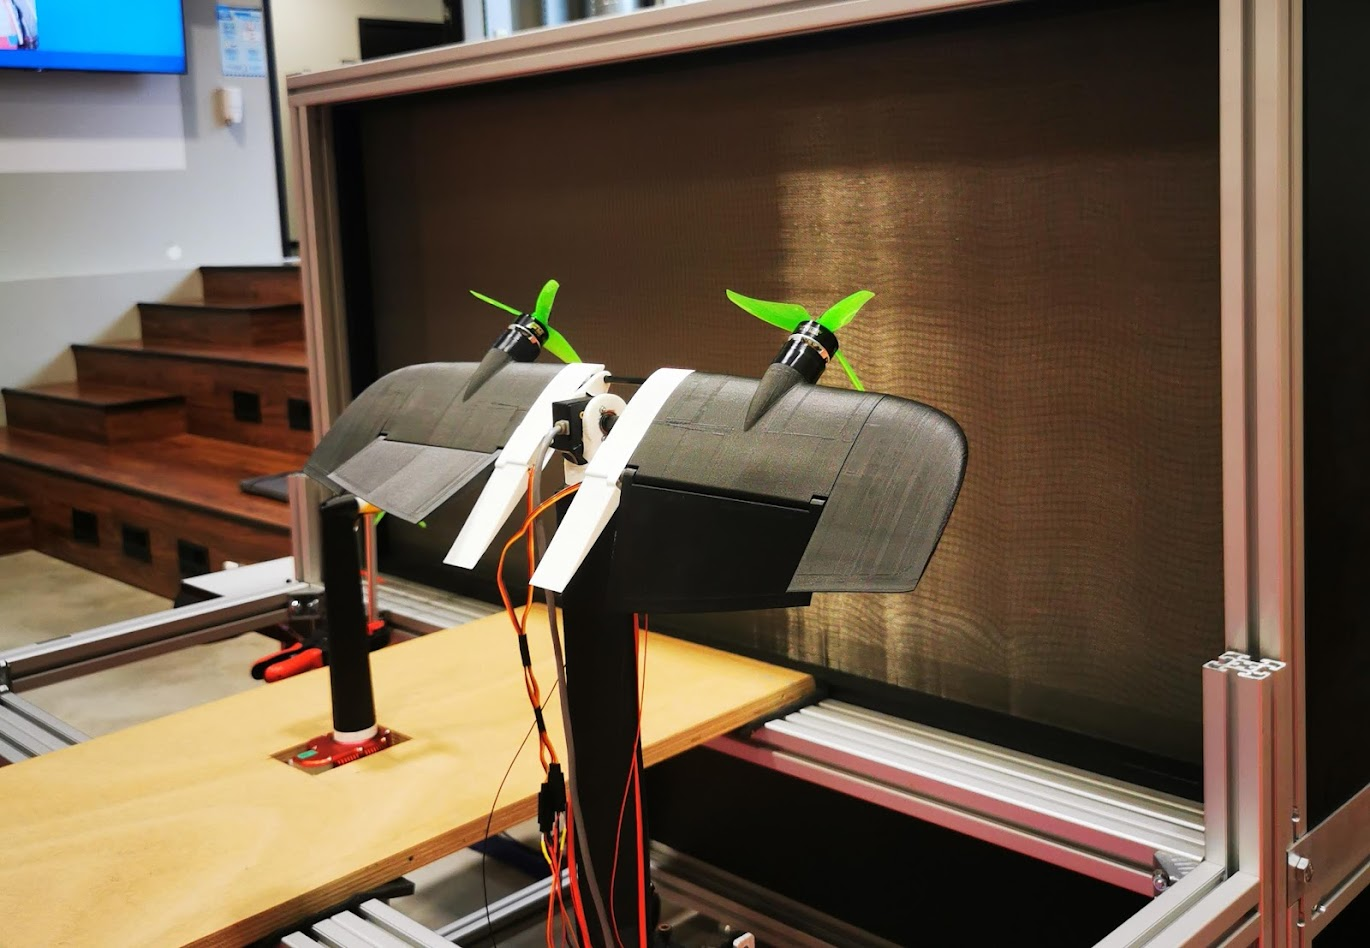
\includegraphics[trim=0cm 5cm 0cm 6cm,clip,width=0.8\columnwidth]{figures/real_test_bench-min.jpg}
    \caption{Modèle de DarkO à un seul degré de liberté devant le \textit{WindShape}.}
    \label{fig:real_test_bench}
\end{figure}
La photo de la figure \ref{fig:real_test_bench} montre le dispositif expérimental dans son environnement de test. Le drone est placé devant une soufflerie ouverte, appelée \textit{WindShape}, qui génère un vent horizontal compris entre 2 et 16 \SI{}{\meter\per\second}. Ainsi, lors de nos tests, nous considérons que la composante verticale du vent est nulle. Le drone est placé au centre du \textit{WindShape}, dans la zone d'écoulement la plus laminaire, tandis que le capteur à fil chaud est placé aussi près que possible du drone. 

La géométrie du dispositif expérimental permet de placer les câbles d'alimentation et de signal près du centre de rotation afin de minimiser leurs effets de friction sur la structure. Malgré cela, le système de rotation interfère inévitablement avec le drone, en créant des forces parasites, notamment de la traînée. La surface projetée de l'articulation étant faible par rapport à la surface de l'aile, la traînée générée par ce support est faible par rapport à la traînée de l'aile et des hélices, et peut donc être négligée.

\begin{figure}[!ht]
    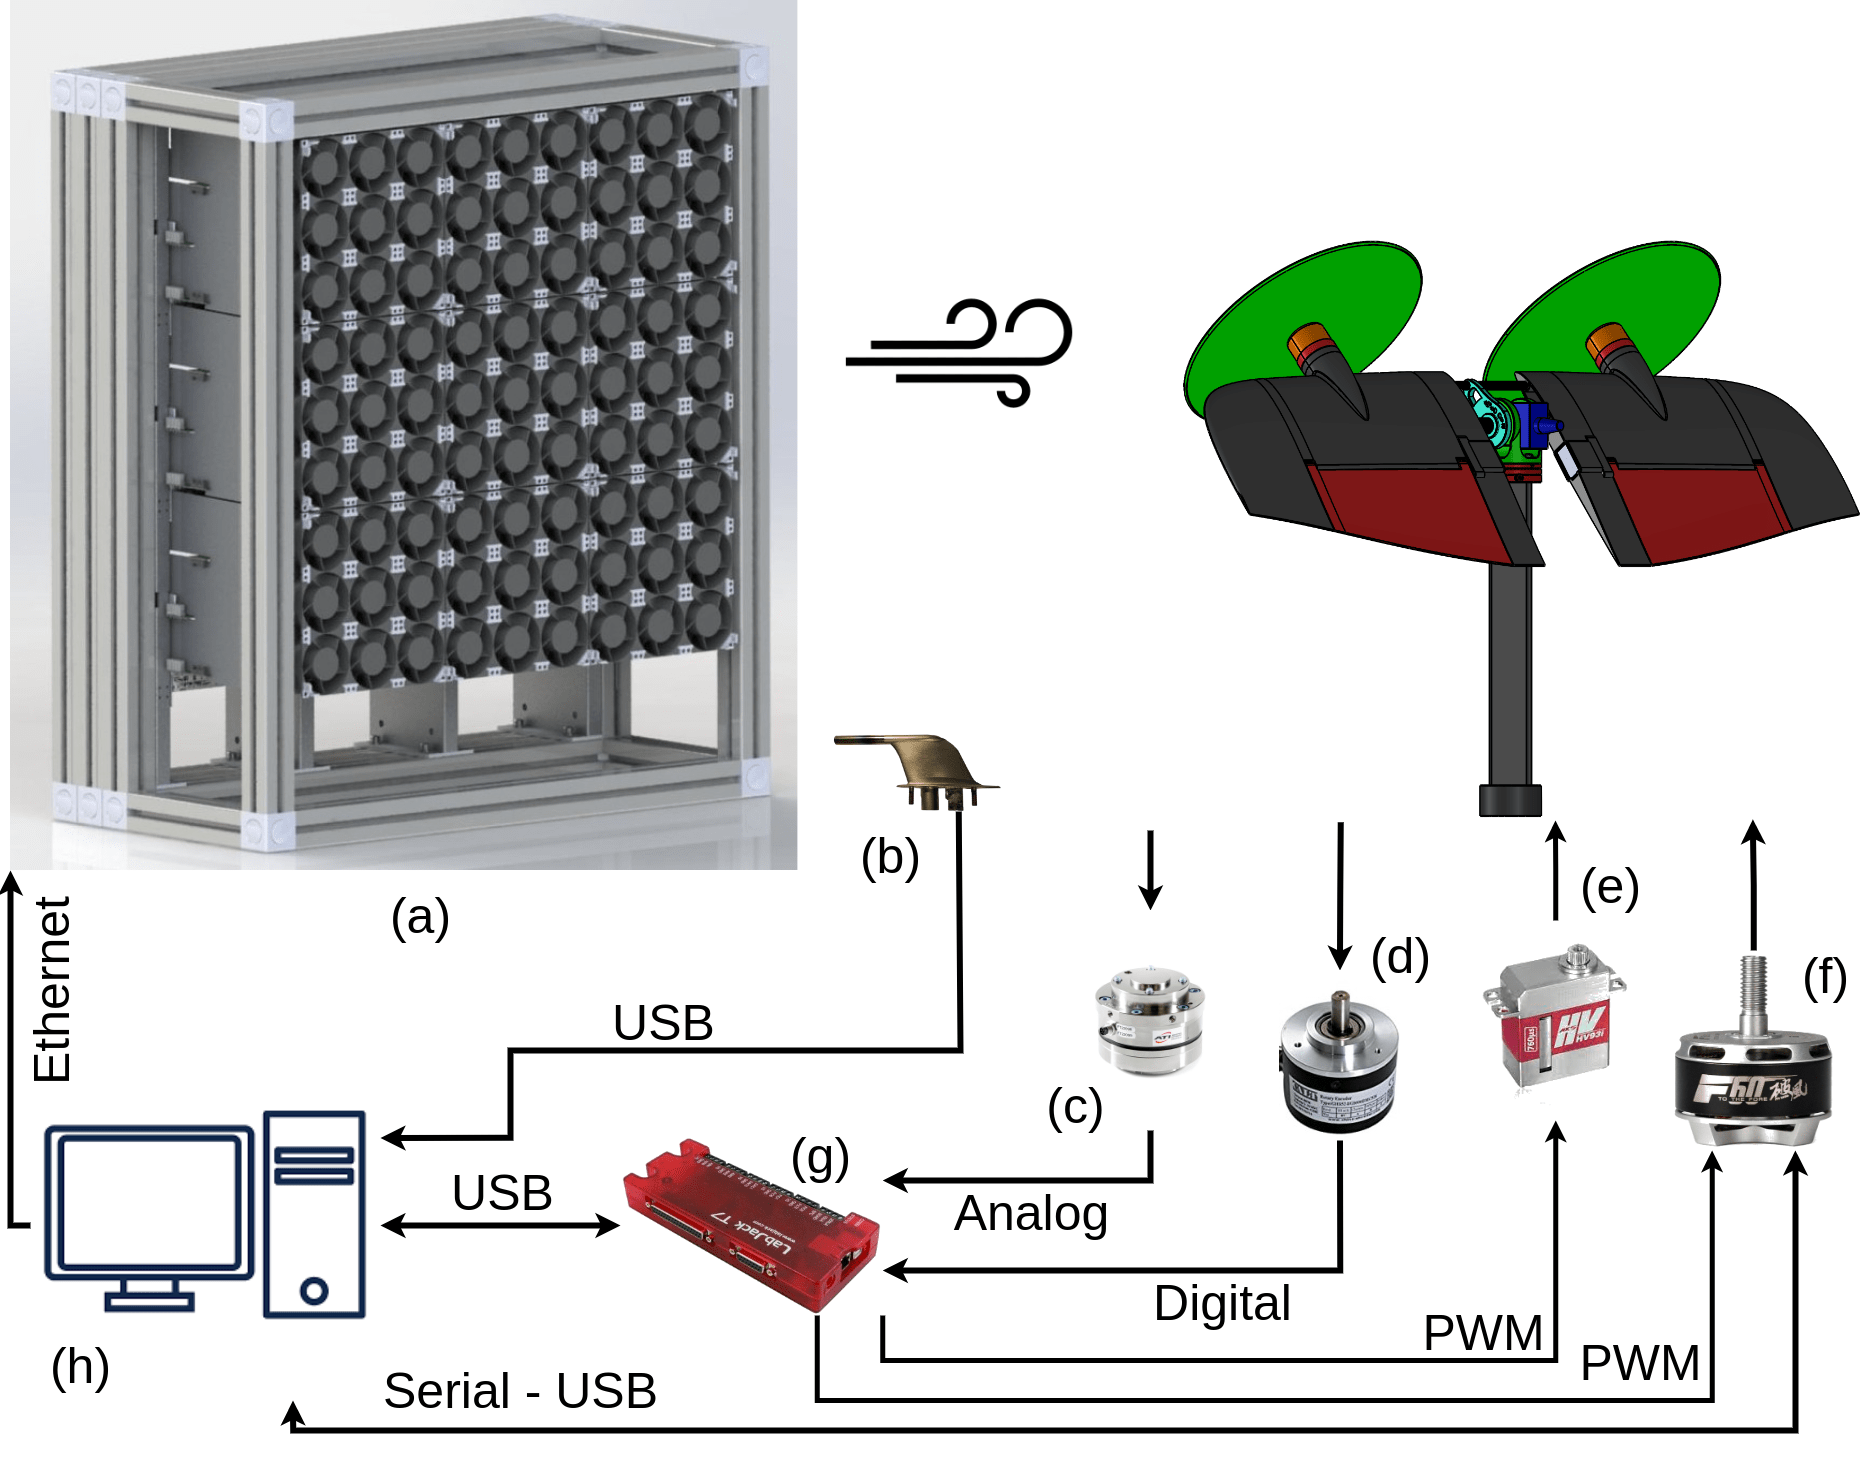
\includegraphics[width=\columnwidth]{figures/maquette-min.png}
    \caption{Architecture d'essai en vol virtuel : \textit{WindShape} (a) ; capteur de vitesse (b) ; capteur de forces et moments (c) ; encodeur rotatif (d) ; servomoteur (e) ; moteur \textit{brushless} + ESC (f) ; LabJack (g) ; ordinateur de contrôle (h)}
    \label{fig:archi}
\end{figure}
Un diagramme schématique des composants du dispositif expérimental et de leur interconnexion est présenté à la Fig. \ref{fig:archi}.

Les moteurs (f) sont alimentés par une batterie externe de 12v 20Ah et les servomoteurs (e) sont alimentés par du 5 V, via un module d'acquisition LabJack T7 \cite[]{LabJack} (g). Le module LabJack (g) concentre la plupart des signaux des capteurs et des actionneurs : six entrées analogiques pour le capteur de force/couple (c), deux entrées numériques en quadrature pour l'encodeur rotatif (d), une entrée analogique (ou une liaison série selon le capteur) pour le capteur de vitesse (b), deux sorties numériques PWM (Pulse Width Modulation) \nomenclature[]{\(PWM\)}{Modulation de largeur d'impulsions (\textit{Pulse Width Modulation})} pour les moteurs (f) et deux sorties numériques PWM pour les servomoteurs (e). 

Les élevons sont commandés par des servomoteurs qui ne fournissent pas de signal de mesure de la position. Nous utilisons donc le point de consigne, en supposant que les actionneurs soient parfaits. Cela est raisonnable en raison de la saturation logicielle imposée à l'entrée des élevons et du dimensionnement correct des servomoteurs par rapport aux forces impliquées. 
Le LabJack (g) possède une interface de programmation d'application (API) \nomenclature[]{\(API\)}{Interface de programmation d'application (\textit{Application Programming Interface})}, permettant une connexion avec un ordinateur. Nous avons développé un code Python qui communique avec le LabJack afin de récupérer les valeurs des capteurs, de calculer la commande à appliquer aux servomoteurs selon le schéma de contrôle présenté ci-dessous et de générer les signaux de sortie pour les servomoteurs. Les données collectées par le LabJack sont enregistrées afin d'être utilisées pour le post-traitement et de générer le graphique présenté dans la section \ref{sec:exp3DOF}. 

Pour générer le vent, nous utilisons un dispositif \textit{WindShape}, lequel dispose également d'une API lui permettant d'être contrôlé via un réseau Ethernet. Le code Python développé peut assigner la vitesse du vent générée par le \textit{WindShape} et donc agir sur le modèle. Il est ainsi possible de tester un ensemble de configurations de vols stationnaires et les transitoires associés dans la même campagne d'essais, sans aucune action sur le modèle. 


\subsection{Simulation des mouvements du drone}
Le prototype étant relié à un support fixe, il n'est pas possible de reproduire expérimentalement le mouvement de translation.  Nous avons donc inclus une simulation logicielle du mouvement en intégrant les mesures de force disponibles au niveau de la fixation. La vitesse de translation (respectivement la position) du drone est obtenue par intégration simple (respectivement double) des données mesurées par le capteur de force. Par souci de simplicité, nous négligeons l'influence aérodynamique de la vitesse (simulée) sur l'aile. En particulier, à partir des équations \eqref{eq:dyna_orig_a} et \eqref{eq:dyna_orig_b}, nous obtenons le modèle simplifié suivant : 
\begin{subequations}\label{eq:accel_sensor}
    \begin{align}
        \boldsymbol{\dot v} &= \boldsymbol{g} + \frac{1}{m}\left( R(\boldsymbol{q})(F\boldsymbol{u} +  D_{\text{f}}(\delta) R^\top(\boldsymbol{q})\lVert \boldsymbol{w} \rVert \boldsymbol{w}) \right)\\
        &= \boldsymbol{g} + \frac{1}{m} \boldsymbol{F}_{meas} \label{eq:sub_accel_sensor},
    \end{align}
\end{subequations}
où $\boldsymbol{F}_{meas}$ représente les forces mesurées par le capteur dans le repère inertiel corrigé du biais. Pour calibrer la correction du biais, lors de l'initialisation, les forces mesurées sont moyennées sur 6000 échantillons, le modèle étant bloqué dans une position stable (angle de tangage à 0°, c'est-à-dire orientation verticale). Pour éliminer le biais de la force mesurée à chaque mesure, nous soustrayons l'effet de la gravité sur le modèle de la mesure. Une masse artificielle $m$ est attribuée à la dynamique du logiciel dans la boucle conformément à \eqref{eq:sub_accel_sensor}, ce qui permet de tester plusieurs configurations afin de mieux apprécier l'influence de la masse du drone sur d'éventuels événements transitoires de saturation. Cela permet d'étudier des scénarios impliquant la masse non négligeable de la batterie, qui n'est pas présente dans notre modèle. Bien que cette manipulation soit aisée, elle ne représente pas parfaitement la réalité car nous ne tenons pas compte de la répartition des masses dans le drone et donc des modifications de l'inertie.
La vitesse et la position transitoire du drone sont ensuite obtenues par intégration numérique simple et double de l'accélération comme dans \eqref{eq:accel_sensor}, en utilisant une intégration numérique trapézoïdale.

\section{Contrôle linéaire, proportionnel-intégral à 3 DOF}
\label{sec:3dofcmd}
Dans la section \ref{sec:ctrl_hyste}, nous avons proposé un bouclage proportionnel stabilisant une position de vol stationnaire en l'absence de vent (sans perturbation). Nous proposons ici une extension incluant une action intégrale, adaptée au fonctionnement avec une perturbation non mesurée représentée par un vent constant. L'objectif est de stabiliser le drone à la position de référence, en rejetant une perturbation de vent constant inconnue.

\subsection{Description du schéma de contrôle}
Nous expérimentons la situation avec le vent agissant uniquement le long de l'axe $x_{i}$, avec le drone orienté vers le vent, c'est-à-dire avec des angles de roulis et de lacet nuls. Dans cette configuration, le vent n'agit que sur la vitesse linéaire le long des axes $x_{b}$ et $z_{b}$, et ne génère qu'un moment autour de l'axe $y_{b}$. Un examen attentif de la commande et des matrices d'entrée des perturbations $\boldsymbol{F}$, $\boldsymbol{M}$ dans \eqref{eq:FandM} suggère une architecture de commande efficace pour rejeter une perturbation constante. En effet, les élevons et les hélices peuvent être utilisés symétriquement pour générer respectivement un moment autour de l'axe $y_{b}$ et une force le long de l'axe $x_{b}$, compensant ainsi l'effet de la perturbation. Néanmoins, il reste une force le long de l'axe $z_{b}$ à compenser et une action intégrale peut converger asymptotiquement vers la force désirée, même avec une perturbation du vent non mesurée $\boldsymbol{w}$. Nous pouvons ainsi stabiliser le drone à une position de vol stationnaire, différente de l'équilibre sans vent. La solution de contrôle exploite le degré de liberté de l'angle de tangage pour compenser l'effet du vent.

\begin{figure}[ht!]
    \centering
    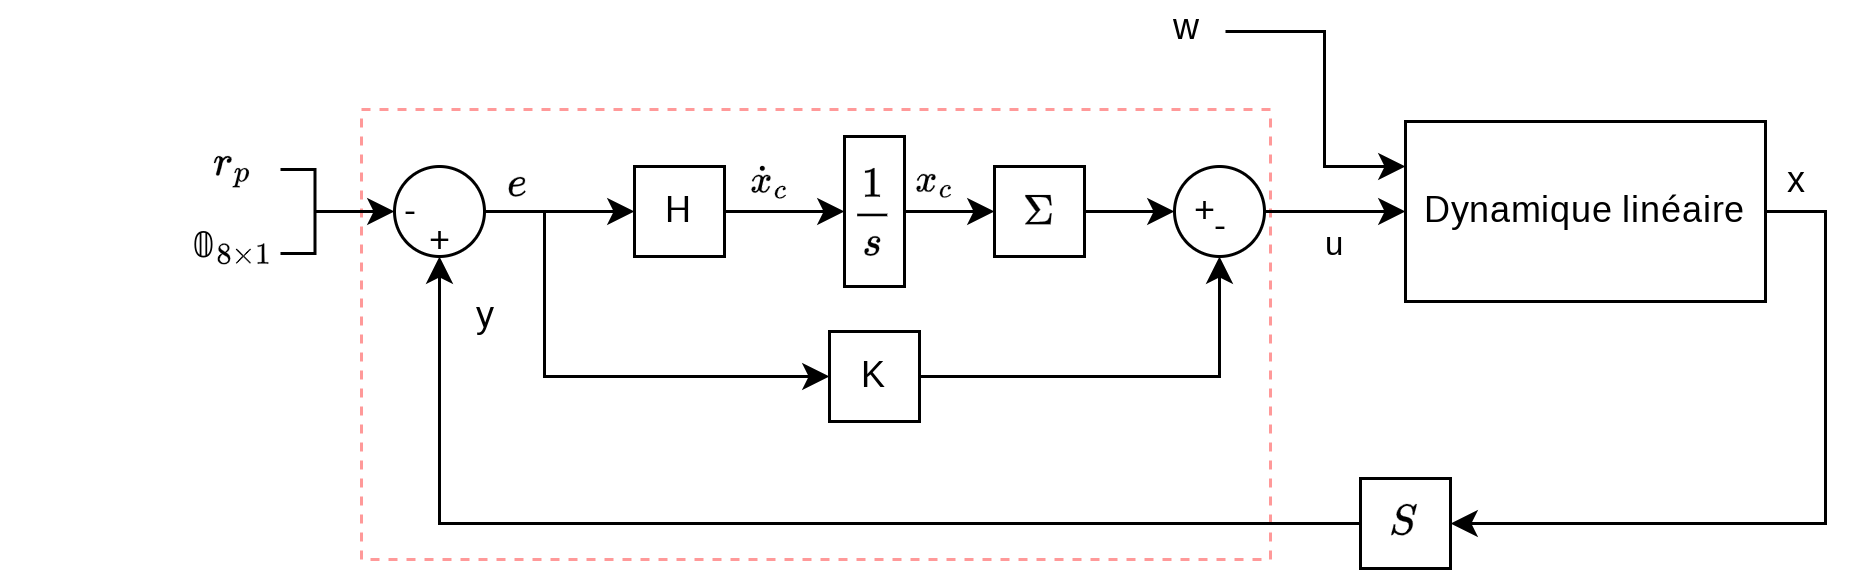
\includegraphics[trim=5cm 0cm 0cm 0cm,clip,width=0.8\columnwidth]{figures/commande_integrale_ACA.png}
    \caption{Schéma de commande linéaire, proportionnel-intégral.}
    \label{fig:commande_int3DOF}
\end{figure}
Le contrôleur proposé, représenté sur la figure \ref{fig:commande_int3DOF}, correspond à :
\begin{subequations}
    \begin{align}
        \label{eq:ctrl3dof}
        \dot{\boldsymbol{x}_{c}} = \boldsymbol{H}(\boldsymbol{y}-\begin{bmatrix}\boldsymbol{r}_{p}\\\mathbb{0}_{8\times 1} \end{bmatrix}), \quad
        \boldsymbol{y} = \boldsymbol{S} \boldsymbol{x},\quad
        \boldsymbol{u} = \Sigma \boldsymbol{x}_{c} + \boldsymbol{K}(\boldsymbol{y}-\begin{bmatrix}\boldsymbol{r}_{p}\\\mathbb{0}_{8\times 1} \end{bmatrix}),\\
        \boldsymbol{S} =\begin{bmatrix} \mathbb{I}_{7} &  \mathbb{0}_{7\times 5} \\
         \mathbb{0}_{4\times 8} &  \mathbb{I}_{4}
          \end{bmatrix}, \quad
          \boldsymbol{\Sigma} = \begin{bmatrix} 1 & 1 & 0 & 0\\ 0 & 0 & 1 & 1\end{bmatrix}^\top,
    \end{align}
\end{subequations}
où $\boldsymbol{x}_{c} \in \mathbb{R}^{2}$ est l'état de l'intégrateur ; $\boldsymbol{r}_{p} \in \mathbb{R}^{3}$ est la référence constante comprenant une position cible pour le mouvement de translation ; $\boldsymbol{S}$ est une matrice de sélection de sortie, qui supprime la composante de l'angle de tangage de la sortie mesurée (n'affectant que la linéarisation par quaternion) pour former $\boldsymbol{y}$ ; $\boldsymbol{\Sigma}$ est une matrice d'allocation d'entrée qui permet d'affecter la première composante de l'état de l'intégrateur à la commande du moteur et la seconde composante à la commande de la gouverne de profondeur. $\boldsymbol{K}$, $\boldsymbol{H}$ sont des gains constants à sélectionner pour que la matrice linéaire de la boucle fermée $\boldsymbol{A}_{cl}$ caractérisant la boucle fermée linéaire soit Hurwitz, afin d'assurer la stabilisation avec la dynamique linéarisée liée au scénario sans vent \eqref{eq:withouwind}.

De manière synthétique, la matrice \eqref{eq:close_matrix} décrit la boucle fermée illustrée à la Fig.~\ref{fig:commande_int3DOF} avec \eqref{eq:ctrl3dof} : un retour de sortie avec 11 sorties, comprenant les trois positions, les trois vitesses linéaires, deux des trois angles ($\epsilon_{1}$ et $\epsilon_{3}$) et les trois vitesses angulaires.
\begin{align} \label{eq:close_matrix}
    \begin{gathered}
        \boldsymbol{A}_{cl} \!= \!
        \begin{bmatrix}\boldsymbol{A} & \mathbb{0}_{12\times 2} \\ \boldsymbol{H}\boldsymbol{S} & \mathbb{0}_{2\times 2}\end{bmatrix} \!- \!\begin{bmatrix}\boldsymbol{G} \\ \mathbb{0}_{2\times 4}\end{bmatrix} \left( \boldsymbol{K} \begin{bmatrix}\boldsymbol{S} & \mathbb{0}_{11\times 2}\end{bmatrix} -  \begin{bmatrix}\mathbb{0}_{4\times 12} & \boldsymbol{\Sigma} \end{bmatrix}\right),
    \end{gathered}
\end{align}
Cette structure peut être considérée comme une solution proportionnelle-intégrale MIMO \nomenclature[]{\(MIMO\)}{Entrées et sorties multiples  (\textit{Multiple-Input Multiple-Output})} résultant d'une observation attentive de la dynamique linéarisée du drone, ce qui permet un nombre minimal d'intégrateurs dans le contrôleur. Ce contrôle devrait permettre de rejeter les perturbations constantes tout en ayant une robustesse satisfaisante. Le gain $\boldsymbol{K}$ correspond au terme proportionnel et le gain $\boldsymbol{H}$ pondère le terme intégral, induisant une convergence vers la cible. La matrice d'allocation $\boldsymbol{\Sigma}$ conduit à une utilisation symétrique des hélices et des ailerons. Il faut alors ajuster $\boldsymbol{K}$ et $\boldsymbol{H}$ pour obtenir un compromis satisfaisant entre robustesse et rejet des perturbations. Nous mettons en œuvre une synthèse multiobjectifs basée sur une méthode d'optimisation $H_{\infty}$, décrite ci-après.

\subsection{Optimisation $H_{\infty}$}
 \label{sec:h_inf3DOF}
Pour effectuer une sélection robuste de $\boldsymbol{K}$ et $\boldsymbol{H}$, nous caractérisons d'abord plusieurs fonctions de transfert dans la figure \ref{fig:commande_int3DOF}.

La sortie de mesure $\boldsymbol{y}$ est utilisée pour la rétroaction, l'entrée $\boldsymbol{u}$ est la somme de l'entrée intégrale $\boldsymbol{\Sigma} \boldsymbol{x}_{c}$ et de l'action proportionnelle $\boldsymbol{K} \boldsymbol{e}$. La sortie $\boldsymbol{z}$ correspond aux signaux de performance de sortie à contrôler ($\boldsymbol{e}$, $\boldsymbol{w}$, $\boldsymbol{u}$, $\boldsymbol{y}$, $\boldsymbol{r}_{p}$). Grâce aux fonctions de pondération $W=\diag (W_{1},..., W_{4})$, la conception de $\boldsymbol{H}$ et $\boldsymbol{K}$ vise à rejeter une perturbation ou un échelon à basse fréquence $\boldsymbol{w}$ agissant sur $\boldsymbol{y}$. L'objectif de la conception est d'amener $\boldsymbol{y}$ à zéro, malgré la perturbation à basse fréquence sur $\boldsymbol{w}$.


Plus précisément, les constantes de pondération sont réglées comme suit :
\begin{align} \label{eq:weight_gain}
    &W_{1} =  0.5, \quad
    W_{2} = 0.5, \quad
    W_{3} = 0.8, \quad 
    W_{4} = 0.5.
\end{align}

\begin{align*} \label{eq:pb_optim}
&\min_{C}\quad \begin{vmatrix}
    \|W_{1} T_{\boldsymbol{r} \rightarrow \boldsymbol{\epsilon}}(P,C)\|\\
    \|W_{2} T_{\boldsymbol{d} \rightarrow \boldsymbol{u}}(P,C)\|\\
    \|W_{3} T_{\boldsymbol{r} \rightarrow \boldsymbol{u}}(P,C)\|\\
    \|W_{4} T_{\boldsymbol{w} \rightarrow \boldsymbol{y}}(P,C)\|
    \end{vmatrix}_{\infty}, \text{ sous condition que } \\ &C \in \mathbb{R}^{11 \times 4} \text{ stabilise } P \text{ en interne.} \numberthis
\end{align*}

Nous avons résolu \eqref{eq:pb_optim} en utilisant le logiciel {\tt Systune} \cite{1576856}. Basé sur l'optimisation non lisse, {\tt Systune} traite plusieurs scénarios non convexes, telle que l'architecture de contrôle structurée où nous optimisons les matrices de gain $\boldsymbol{K}$, $\boldsymbol{H}$. L'algorithme d'optimisation renvoie la sélection optimisée suivante :

\begin{align}\label{eq:HK}
\begin{bmatrix}
    \boldsymbol{H}\\ \hline \boldsymbol{K }
\end{bmatrix} = \smallmat{
\shortminus1.902 & 0 & 7.201 & \shortminus9.043  & 0 & 33.244 & 0 & 0 & 0 & 4.696  & 0 \\ 
0.425 & 0 & \shortminus1.620 & 2.024  & 0 & \shortminus7.480 & 0 & 0 & 0 & \shortminus1.045  & 0 \\  \hline
0.035 & 0 & \shortminus0.728 & \shortminus1.853  & 0 & \shortminus4.445 & 0 & 0 & 0 & \shortminus0.323  & 0 \\ 
0.035 & 0 & \shortminus0.728 & \shortminus1.853  & 0 & \shortminus4.445 & 0 & 0 & 0 & \shortminus0.323  & 0 \\ 
0.217  & 0 & \shortminus0.164  & 1.074 & 0 & \shortminus0.527 & 0 & 0 & 0 & \shortminus0.773 & 0 \\ 
0.217  & 0 & \shortminus0.164  & 1.074 & 0 & \shortminus0.527 & 0 & 0 & 0 & \shortminus0.773 & 0  
}.
\end{align}
Nous obtenons une abscisse spectrale en boucle fermée pour $\boldsymbol{A}_{cl}$ dans \eqref{eq:close_matrix} valant $\alpha = -0.2381$.

\section{Résultats}
\label{sec:exp3DOF}
La figure~\ref{fig_exp_centrage_arr} montre le résultat de la boucle fermée de la figure~\ref{fig:commande_int3DOF} avec la sélection des gains \eqref{eq:HK} et une valeur constante et croissante par morceaux du vent horizontal $w$ (dernier graphique). 
Malgré quelques oscillations, le drone maintient sa position en dépit du vent, en inclinant convenablement l'angle de tangage. Les oscillations expérimentales sont absentes de nos simulations, ce qui suggère la présence de phénomènes non modélisés.
Nous observons également un comportement qui pourrait être important pour de futures recherches : le drone semble se stabiliser plus facilement le long de l'axe vertical que le long de l'axe horizontal. 

Comme prévu, lorsque le vent augmente, l'angle d'inclinaison diminue, ce qui modifie la poussée nécessaire et la déflexion des élevons. En effet, le vent génère de la portance sur les ailes, ce qui compense l'effet de la gravité, et donc la poussée nécessaire devient plus faible.
Pour chaque valeur de $w$, le modèle converge vers un équilibre, dont la caractérisation mathématique précise est détaillée dans \ref{sec:eq_vent}. Il est donc nécessaire d'étendre la robustesse du contrôleur en effectuant une optimisation multimodèle du contrôleur (décrite dans \ref{sec:h_inf6DOF_multi}). Il est également possible de supprimer les contraintes sur la structure du contrôleur afin de lui donner plus de degrés de liberté dans l'optimisation.

La vidéo de la maquette, avec les résultats expérimentaux est, disponible via le lien : \url{https://youtu.be/ce4_FUzeVzI}.

\begin{figure}[!ht]
   \centering
    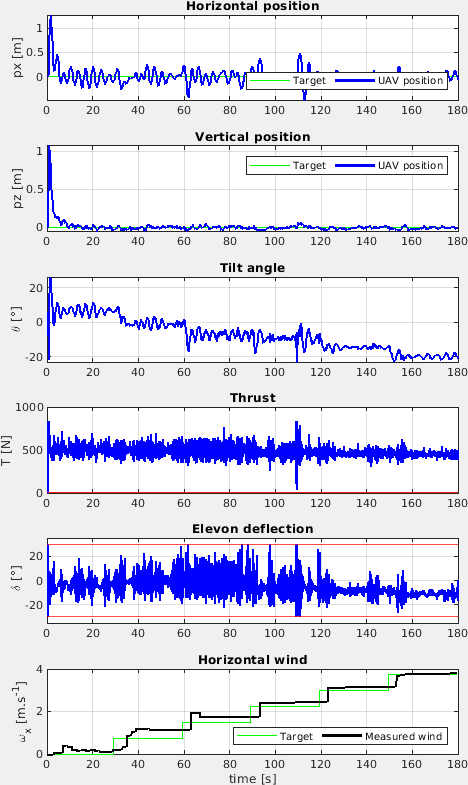
\includegraphics[width=0.7\columnwidth]{figures/exp.png}
    \caption{Résultats expérimentaux.}
    \label{fig_exp_centrage_arr}
\end{figure}

\section{Conclusion du Chapitre \ref{chap:3DOF}}
Nous avons décrit une maquette permettant de simuler le vol d'un drone convertible, DarkO, en soufflerie. L'objectif de cette maquette est de tester le système de contrôle sur une représentation fidèle de la dynamique longitudinale, tout en simulant la dynamique de translation. Nous avons également présenté un contrôleur linéaire de sortie basé sur une architecture proportionnelle-intégrale pour la stabilisation du vol stationnaire dans des conditions de vent constant. Les gains du contrôleur ont été obtenus à l'aide d'une optimisation non convexe. Les résultats des essais expérimentaux montrent qu'il est possible de stabiliser l'équilibre en vol stationnaire dans la plage de vitesse du vent testée. 

Toutefois, d'autres architectures de contrôle devraient être étudiées à l'avenir pour traiter les oscillations indésirables. Ces résultats indiquent qu'il est nécessaire de tester cette architecture de commande sur un modèle complet à six degrés de liberté, dans des conditions similaires de vent.


% \subsection{\texorpdfstring{$H_{\infty}$}{H {infty}}-based optimization}



% From the Nyquist criterion, we know that the margin corresponds to the minimal distance between the singularity (real point -1) and the product between the controller (C) and the plant (P). Consequently, we define the input modulus margin as $MM_{u} =\min_{\omega\in R}|1-CP|$ and the output modulus margin as $MM_{y} =\min_{\omega\in R}| 1-PC |$ for a positive feedback. We first introduce the output sensitivity function  $T_{r \rightarrow \epsilon}=S_{y}=(1-PC)^{-1}$, so that $\lVert S_{y} \rVert_{\infty}=MM_{y}^{-1}$ and the input sensitivity function $T_{d \rightarrow u}=S_{u}=(1-CP)^{-1}$, so that $\lVert S_{u} \rVert_{\infty}=MM_{u}^{-1}$. Consequently, the minimization of the  $H_{\infty}$-norm of $S_{u}$ or $S_{y}$, leads to improving the input and output modulus margins. As our system is MIMO, we give importance to both the input and output sensitivity functions, because they do not commute. We also define the transfer functions $T_{r \rightarrow u}= CS_{y} = S_{u}C$ and $T_{w \rightarrow y}$. In order to guarantee a satisfactory trade-off between robustness and performance, we select the weighting functions $W_{1}$, $W_{2}$, $W_{3}$ and $W_{4}$ linked to $\lVert W_{1} T_{r \rightarrow \epsilon}(s)\rVert_{\infty} \leq 1 $ and $\lVert W_{2} T_{d \rightarrow u}(s)\rVert_{\infty} \leq 1 $, corresponding to robustness margins at the inputs and outputs, $\lVert W_{3} T_{r \rightarrow u}(s)\rVert_{\infty} \leq 1 $ limiting the control effort, $\lVert W_{4} T_{w \rightarrow y}(s)\rVert_{\infty} \leq 1 $ ensuring suitable wind disturbance rejection. Specifically, the weighting functions are tuned as
% \begin{align}
%     &W_{1} =  0.5, \quad
%     W_{2} = 0.5, \quad
%     W_{3} = 0.8, \quad 
%     W_{4} = 0.5.
% \end{align}
% The values of $W_{1}$ and $W_{2}$ ensure $MM_{u} >  6~dB$ and $MM_{y} >  6~dB$, $ W_{3}$ and $W_{4}$ are tuned to obtain a satisfactory trade-off between the different specifications. The weight $ W_{4} $  allows managing, among other things, the speed of the rejection.
% With selections \eqref{eq:weight_gain}, we cast the design problem for $K$ and $H$ as an $H_{\infty}$ synthesis under order constraint, providing good input and output specifications for the closed loop:
% \begin{align*} \label{eq:pb_optim}
% &\min_{C}\quad \begin{Vmatrix}
%     W_{1} T_{r \rightarrow \epsilon}(P,C)\\
%     W_{2} T_{d \rightarrow u}(P,C)\\
%     W_{3} T_{r \rightarrow u}(P,C)\\
%     W_{4} T_{w \rightarrow y}(P,C)
%     \end{Vmatrix}_{\infty}, \text{ subject to} \\ &C \in \mathbb{R}^{11 \times 4} \text{ stabilizes } P \text{ internally,} \numberthis
% \end{align*}

% where $P$ is the augmented plant containing the integral action and the linearized UAV dynamics. In addition, we impose constraints on the gains $K$ and $H$ ensuring that the closed loop with experimental device only evolves in the ($x$,$z$) plane, compatibly.









